\section{Theory}
\subsection{Theoretical Exercises}
\subsubsection[Origin of the 21 cm HI-Line]{Origin of the \SI{21}{cm} \ce{H_I}-Line}
The \SI{21}{cm} \ce{H_I}-Line refers to electromagnetic radiation emitted from atomic hydrogen. It has a wavelength of \SI{21.11}{cm} (that is \SI{1420.03}{\mega\hertz}) \cite[Ch 3.1]{srt}.

This emission is caused by a transition from the $\ce{S_{\frac{1}{2}}(F=1)}$ to the $\ce{S_{\frac{1}{2}}(F=0)}$ state, meaning that the nuclear spin and electron spin transition from parallel to antiparallel.
The $\ce{S_{\frac{1}{2}}(F=1)}$-state has a half live of about 8 million years, but the sheer amount of atomic hydrogen makes the line visible nonetheless. \cite[Ch. 13.1]{wilson_tools_2009}

The main reason for interest in specifically this frequency is the aforementioned atomic hydrogen, but there are other sources that can emit at this wavelength, some of them are: \cite[11.1-11.4]{wilson_tools_2009}
\begin{itemize}
    \item The sun
    \item Thermal radiation from molecular hydrogen
    \item Ionized stellar winds
    \item Supernovae
\end{itemize}
\subsubsection{Angular resolution of the SRT}\label{sec:ang_res}
Using the equation relating the effective area $A_e$ and the wavelength $\lambda$ \cite[p. 149]{wilson_tools_2009}
\begin{equation}
    A_e \Omega_A = \lambda^2
\end{equation}
and the definitions of the effective area and the geometric area \cite[p. 148]{wilson_tools_2009}
\begin{equation}
    A_e = \eta A_g \qquad A_g = \pi \left( \frac{d}{2} \right)^2 \label{eq:A_e}
\end{equation}
we can then solve for the effective antenna area.
\begin{equation}
    \Omega_A = \frac{\lambda^2}{A_g \eta} \label{eq:Omega_A}
\end{equation}


To compute an approximation of the full width at half maximum $\theta$ (FWHM) we can approximate the aperture as gaussian \cite[p. 2]{srt} and note the following properties.
\begin{equation}
    \Omega_A \approx \int_{4\pi } d\Omega\, \exp{\left( -\frac{\vartheta^2}{2\sigma^2} \right)} \approx 2\pi \int_0^{\infty} d\vartheta \, \vartheta \exp{\left( -\frac{\vartheta^2}{2\sigma^2} \right)} = 2\pi \sigma^2
    \label{eq:gauss_integral}
\end{equation}
\begin{equation}
    \exp{\left( -\frac{(\theta/2)^2}{2\sigma^2}\right)} = \frac{1}{2} \quad \implies \quad \theta = 2 \sqrt{2\ln{2}} \sigma \label{eq:fwhm_sigma}
\end{equation}
using Eq. \eqref{eq:gauss_integral} and Eq. \eqref{eq:fwhm_sigma} we can solve for $\Omega_A$ in terms of $\theta$
\begin{equation}
    \Omega_A = \frac{\pi}{4\ln{2}} \theta \approx 1.133 \, \theta^2 \label{eq:Omega_A_fwhhm}
\end{equation}
Notice that this is consistent with \cite[p.178 (8.13)]{wilson_tools_2009}

Equating Eq. \eqref{eq:Omega_A} and Eq. \eqref{eq:Omega_A_fwhhm} and then solving for $\theta$ we get an expression for the expected FWHM.
\begin{equation}
    \theta = \frac{4}{\pi} \sqrt{\frac{\ln{2}}{\eta}}\frac{\lambda}{d} \label{eq:fwhm}
\end{equation}

To compute the FWHM we need the diameter of the SRT which is $d = \SI{4}{m}$ \cite[p. 4]{srt}, and the antenna efficiency which is $\eta = 0.5$ \cite[p. 2]{srt}.
Unfortunately we cannot reasonably estimate an error for the antenna efficiency $\eta$, we suspect however that the error of the antenna efficiency dominates here.
Therefore we will waive a proper error discussion at this point, and work with exact values.

We can then obtain the values shown in Table \ref{tab:ang_res}.
\begin{table}[H]
    \centering
    \begin{tabular}{rrrr}
        \toprule
        FWHM $\theta$ [\si{\degree}] & Wavelength $\lambda$ [\si{cm}] & Frequency [\si{\giga \hertz}]\\
        \midrule
        \num{4.533} & \num{21.11} & \num{1.420}\\
        \num{0.688} & \num{0.30} & \num{10.000}\\
        \bottomrule
    \end{tabular}
    \caption{Angular resolution of the SRT at different frequencies}
    \label{tab:ang_res}
\end{table}
\subsubsection{Antenna, brightness and noise temperature}

\subsubsection{Temperature conversion}

\subsubsection{Expected temperature of the sun}\label{sec:temp}
If we assume that the sun is a black body at the wavelength of \SI{1.42}{\giga\hertz} we expect the sun to have a brightness temperature of $T_{\odot} = \SI{5778}{\kelvin}$ \cite[p. 211]{durandi_formeln_2011}.
In Figure \ref{fig:sun_temp_theory} we can see however, that the sun has a brightness temperature of 100'000 \si{\kelvin} up to 10 million \si{\kelvin}.
\begin{figure}[H]
    \centering
    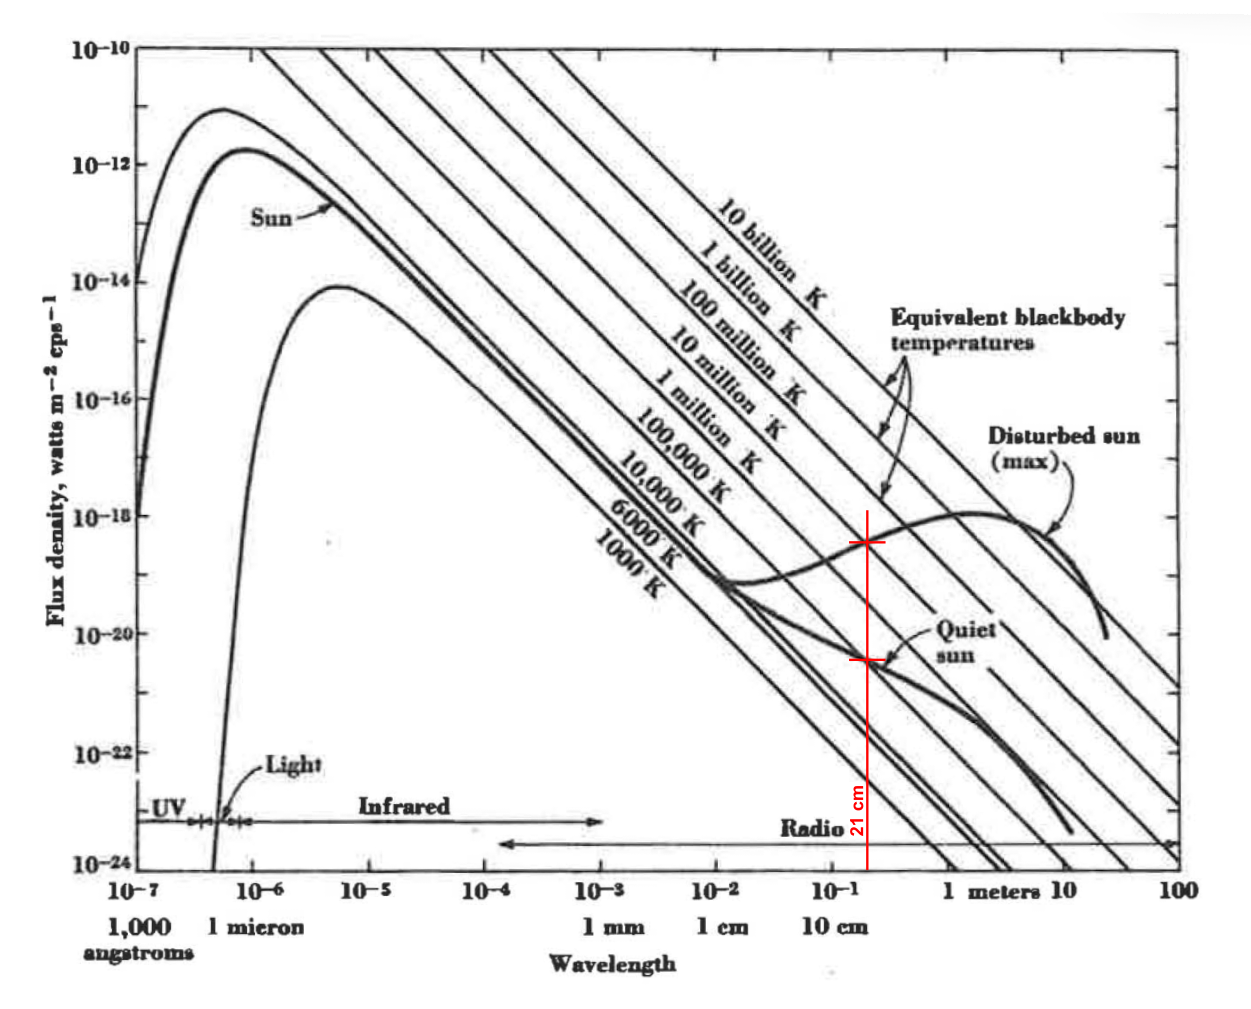
\includegraphics[width=0.6\textwidth]{assets/SunBrightnessTheory.png}
    \caption{Wavelength dependence of the Brightness temperature of the sun \cite[p.8-45 Fig. 8-34]{kraus_radio_1986}}
    \label{fig:sun_temp_theory}
\end{figure}

\subsubsection{Influence of elevation angle}
At a frequency of \SI{1.42}{\giga\hertz} we don't expect a significant influence of the elevation angle on the measured brightness temperature, since the atmosphere is transparent at this wavelength.
The frequency of \SI{22}{\giga\hertz} is however very close to an absorption band caused by water vapor \ce{H_2O} at \SI{22.2}{\giga\hertz}.
We can make a reasonable but naive model of the attenuation at this frequency by considering that the attenuation is exponential in the distance traveled through the atmosphere.
Ignoring the curvature of the earth, the distance traveled through the atmosphere can be computed trigonometrically. We can then model the attenuation $\alpha$ with Eq.\eqref{eq:attenuation}.
\begin{equation}
    \alpha = C_1 \exp{\left( - C_2 \frac{1}{\abs{\cos{\theta}}} \right)} \label{eq:attenuation}
\end{equation}

\subsubsection{Doppler shift}

\subsection{Rotation of the Milky Way}
